\definecolor{promptbg}     {HTML}{FAFAF8}
\definecolor{promptborder} {HTML}{C8C6BC}
\definecolor{headerbg}     {HTML}{EEEDFE}
\definecolor{headerborder} {HTML}{534AB7}
\definecolor{exbg}         {HTML}{E1F5EE}
\definecolor{exborder}     {HTML}{0F6E56}
\definecolor{querybg}      {HTML}{FAEEDA}
\definecolor{queryborder}  {HTML}{854F0B}
\definecolor{rolecolor}    {HTML}{3C3489}
\definecolor{commentcolor} {HTML}{888780}
\definecolor{excolor}      {HTML}{085041}
\definecolor{querycolor}   {HTML}{633806}
\definecolor{keycolor}     {HTML}{185FA5}
\definecolor{valcolor}     {HTML}{2C2C2A}
\definecolor{divcolor}     {HTML}{D3D1C7}

\newcommand{\sectionpill}[4]{%
  \tikz[baseline=-0.6ex]\node[
    rectangle, rounded corners=3pt,
    fill=#1, draw=#2, line width=0.4pt,
    inner xsep=5pt, inner ysep=2pt,
    font=\scriptsize\bfseries, text=#4
  ] {#3};%
}

%% Outer box width
\newlength{\promptwidth}
\setlength{\promptwidth}{13.0cm}

%% Inner body width = promptwidth - 2 * horizontal padding (12pt each side)
\newlength{\bodywidth}
\setlength{\bodywidth}{12.32cm}

\newcommand{\promptrule}{%
  \textcolor{divcolor}{\rule{\bodywidth}{0.3pt}}%
}

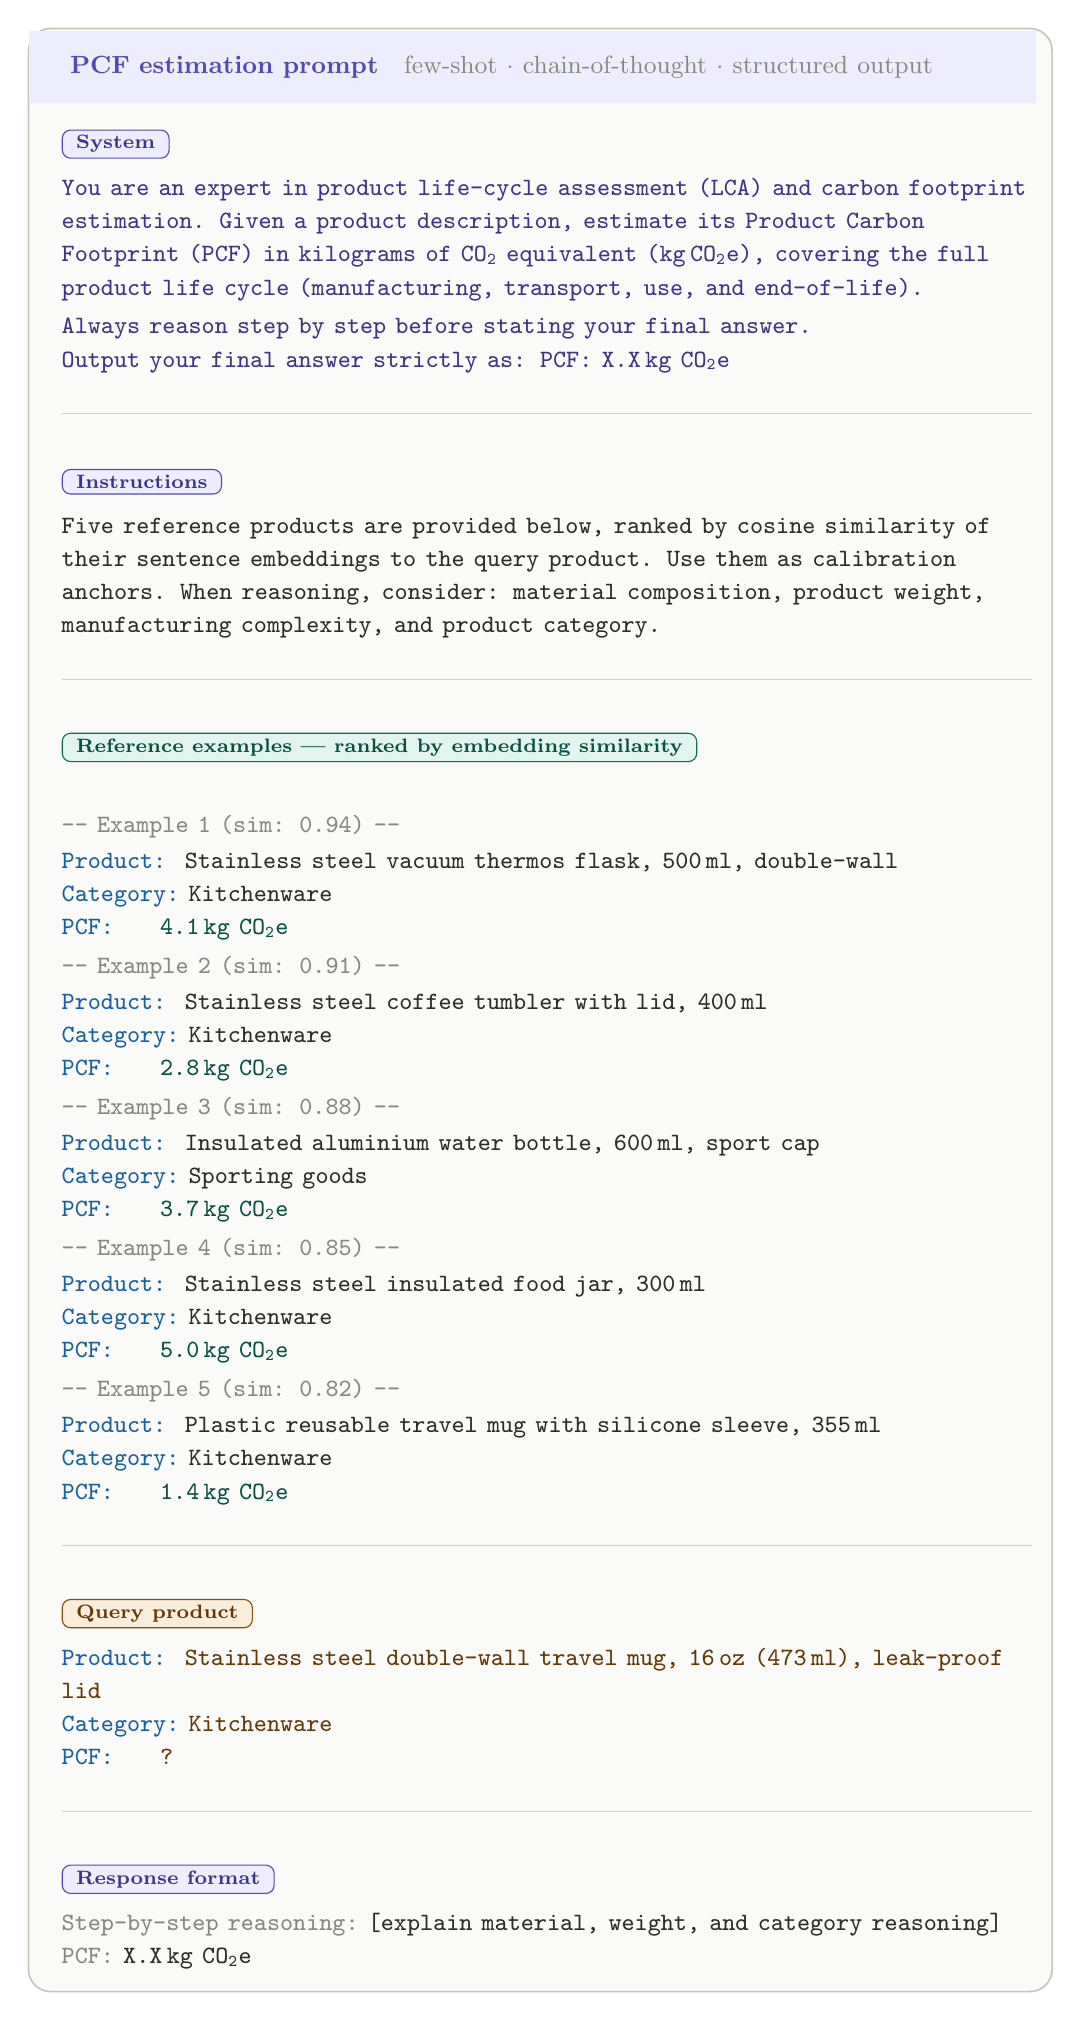
\begin{tikzpicture}
\node[
  rectangle,
  rounded corners=8pt,
  fill=promptbg,
  draw=promptborder,
  line width=0.6pt,
  inner sep=0pt,
  text width=\promptwidth,
  align=left
] (prompt) {%

  %% ── Header band: colorbox must equal promptwidth exactly ─────────
  \noindent\colorbox{headerbg}{%
    \hspace{12pt}%
    \begin{minipage}[c]{\dimexpr\promptwidth-24pt\relax}%
      \vspace{6pt}%
      {\small\textbf{\textcolor{headerborder}{PCF estimation prompt}}%
      \quad\textcolor{commentcolor}{few-shot $\cdot$ chain-of-thought $\cdot$ structured output}}%
      \vspace{6pt}%
    \end{minipage}%
    \hspace{0pt}%
  }%

  %% ── Body ─────────────────────────────────────────────────────────
  \hspace{12pt}%
  \begin{minipage}[t]{\bodywidth}
  \vspace{8pt}

  \sectionpill{headerbg}{headerborder}{System}{rolecolor}\\[4pt]
  {\small\ttfamily\textcolor{rolecolor}{%
    You are an expert in product life-cycle assessment (LCA) and
    carbon footprint estimation. Given a product description, estimate
    its Product Carbon Footprint (PCF) in kilograms of CO\textsubscript{2}
    equivalent (kg\,CO\textsubscript{2}e), covering the full product life cycle
    (manufacturing, transport, use, and end-of-life).\\[2pt]
    Always reason step by step before stating your final answer.\\
    Output your final answer strictly as: \textbf{PCF: X.X\,kg CO\textsubscript{2}e}
  }}
  \vspace{5pt}\\
  \promptrule\\
  \vspace{3pt}

  \sectionpill{headerbg}{headerborder}{Instructions}{rolecolor}\\[4pt]
  {\small\ttfamily\textcolor{valcolor}{%
    Five reference products are provided below, ranked by cosine
    similarity of their sentence embeddings to the query product.
    Use them as calibration anchors. When reasoning, consider:
    material composition, product weight, manufacturing complexity,
    and product category.%
  }}
  \vspace{5pt}\\
  \promptrule\\
  \vspace{3pt}

  \sectionpill{exbg}{exborder}{Reference examples --- ranked by embedding similarity}{excolor}\\[4pt]

  {\small\ttfamily%
    \textcolor{commentcolor}{-- Example 1 (sim: 0.94) --}\\[1pt]
    \textcolor{keycolor}{Product:}\ \ \textcolor{valcolor}{Stainless steel vacuum thermos flask, 500\,ml, double-wall}\\
    \textcolor{keycolor}{Category:}\ \textcolor{valcolor}{Kitchenware}\\
    \textcolor{keycolor}{PCF:}\ \ \ \ \ \textcolor{excolor}{\textbf{4.1\,kg CO\textsubscript{2}e}}
  }\\[2pt]
  {\small\ttfamily%
    \textcolor{commentcolor}{-- Example 2 (sim: 0.91) --}\\[1pt]
    \textcolor{keycolor}{Product:}\ \ \textcolor{valcolor}{Stainless steel coffee tumbler with lid, 400\,ml}\\
    \textcolor{keycolor}{Category:}\ \textcolor{valcolor}{Kitchenware}\\
    \textcolor{keycolor}{PCF:}\ \ \ \ \ \textcolor{excolor}{\textbf{2.8\,kg CO\textsubscript{2}e}}
  }\\[2pt]
  {\small\ttfamily%
    \textcolor{commentcolor}{-- Example 3 (sim: 0.88) --}\\[1pt]
    \textcolor{keycolor}{Product:}\ \ \textcolor{valcolor}{Insulated aluminium water bottle, 600\,ml, sport cap}\\
    \textcolor{keycolor}{Category:}\ \textcolor{valcolor}{Sporting goods}\\
    \textcolor{keycolor}{PCF:}\ \ \ \ \ \textcolor{excolor}{\textbf{3.7\,kg CO\textsubscript{2}e}}
  }\\[2pt]
  {\small\ttfamily%
    \textcolor{commentcolor}{-- Example 4 (sim: 0.85) --}\\[1pt]
    \textcolor{keycolor}{Product:}\ \ \textcolor{valcolor}{Stainless steel insulated food jar, 300\,ml}\\
    \textcolor{keycolor}{Category:}\ \textcolor{valcolor}{Kitchenware}\\
    \textcolor{keycolor}{PCF:}\ \ \ \ \ \textcolor{excolor}{\textbf{5.0\,kg CO\textsubscript{2}e}}
  }\\[2pt]
  {\small\ttfamily%
    \textcolor{commentcolor}{-- Example 5 (sim: 0.82) --}\\[1pt]
    \textcolor{keycolor}{Product:}\ \ \textcolor{valcolor}{Plastic reusable travel mug with silicone sleeve, 355\,ml}\\
    \textcolor{keycolor}{Category:}\ \textcolor{valcolor}{Kitchenware}\\
    \textcolor{keycolor}{PCF:}\ \ \ \ \ \textcolor{excolor}{\textbf{1.4\,kg CO\textsubscript{2}e}}
  }
  \vspace{5pt}\\
  \promptrule\\
  \vspace{3pt}

  \sectionpill{querybg}{queryborder}{Query product}{querycolor}\\[4pt]
  {\small\ttfamily%
    \textcolor{keycolor}{Product:}\ \ \textcolor{querycolor}{\textbf{Stainless steel double-wall travel mug, 16\,oz (473\,ml), leak-proof lid}}\\
    \textcolor{keycolor}{Category:}\ \textcolor{querycolor}{\textbf{Kitchenware}}\\
    \textcolor{keycolor}{PCF:}\ \ \ \ \ \textcolor{querycolor}{\textbf{?}}
  }
  \vspace{5pt}\\
  \promptrule\\
  \vspace{3pt}

  \sectionpill{headerbg}{headerborder}{Response format}{rolecolor}\\[4pt]
  {\small\ttfamily%
    \textcolor{commentcolor}{Step-by-step reasoning:}\ \textcolor{valcolor}{[explain material, weight, and category reasoning]}\\
    \textcolor{commentcolor}{PCF:}\ \textcolor{valcolor}{X.X\,kg CO\textsubscript{2}e}
  }
  \vspace{8pt}

  \end{minipage}
  \hspace{12pt}%
};
\end{tikzpicture}